\section{Base Teórica}

La planificación es un componente fundamental del sistema operativo que se encarga de asignar tiempo de procesamiento a los diferentes hilos y procesos que se ejecutan en un sistema. En este capítulo se presentará la información necesaria para comprender la planificación a corto plazo, con un enfoque específico en el sistema operativo FreeBSD y su planificador 4BSD. Se describirán los conceptos fundamentales de procesos e hilos, incluyendo su estructura y estados, y se explicará cómo el planificador toma decisiones sobre cuál hilo o proceso debe ejecutarse en un momento dado. Además, se examinarán en detalle las operaciones de cambio de contexto, encolado, elección del procesador y remoción de hilos de la cola, que son funciones clave del planificador 4BSD. Con esta base teórica, se sentarán las bases para entender cómo funciona el planificador de FreeBSD y cómo puede ser mejorado.


\subsection{Procesos e hilos}

En sistemas operativos, los procesos son entidades aisladas que representan la ejecución de una tarea o aplicación en particular. Cada proceso cuenta con su propio espacio de direcciones, que es un área reservada de memoria virtual donde se aloja el código del programa, las variables y los recursos necesarios para su ejecución. Además, disponen de acceso a los recursos del kernel a través de llamadas a sistemas.\par

Cada proceso puede alojar uno o varios hilos de ejecución. Estos son subunidades dentro de un proceso que pueden ejecutarse de manera independiente, y comparten los recursos del mismo. Cada hilo se corresponde con un procesador virtual que cuenta con su propio contexto y un stack de ejecución que se aloja en el espacio de direcciones del proceso.\par

El kernel del sistema operativo soporta la ilusión de ejecución concurrente de múltiples procesos al repartir los recursos del sistema entre los procesadores que están listos para ejecutar.\par

Los hilos de un proceso pueden operar en dos modos distintos: modo usuario y modo kernel. En modo usuario, el hilo ejecuta el código de la aplicación sin permisos elevados. Cuando el hilo necesita acceder a algún recurso o servicio del sistema operativo, se realiza una transición al modo kernel mediante un mecanismo de protección. En este modo, el hilo obtiene acceso a recursos del kernel, como registros por hardware, el contador de programa y el puntero al stack, lo que le permite realizar tareas que no están disponibles en modo usuario.\par

\subsubsection{Estructura de los procesos}
Cada proceso en el sistema recibe un identificador único llamado identificador de proceso (PID). Los PID son el mecanismo común utilizado por las aplicaciones y el kernel para hacer referencia a los procesos. Existen dos identificadores que son de especial importancia para cada proceso: el PID del proceso en sí, y el PID del proceso padre.\par

Los procesadores poseen diversas categorías de información que los definen y describen su comportamiento y funcionalidad. La estructura simplificada se puede observar en la Figura \ref{fig:process_state}. El objetivo es permitir múltiples hilos que compartan un espacio de direcciones y otros recursos.  Algunas de estas categorías son:\par

\begin{itemize}
    \item Identificación del grupo de procesos: el grupo de procesos y la sesión a la que pertenece el proceso.
    \item Credenciales de usuario: los identificadores reales, efectivos y guardados de usuario y grupo.
    \item Gestión de memoria: la estructura que describe la asignación del espacio de direcciones virtuales utilizado por el proceso.
    \item Descriptores de archivos: una matriz de punteros a entradas de archivos indexadas por los descriptores de archivos abiertos del proceso; también, las banderas de archivos abiertos y el directorio actual.
    \item Vector de llamadas al sistema: la asignación de números de llamadas al sistema a acciones.
    \item Contabilidad de recursos: las estructuras de límite de recursos (rlimit) que describen la utilización de los recursos proporcionados por el sistema.
    \item Estadísticas: estadísticas recopiladas mientras el proceso se está ejecutando que se informan cuando sale y se escriben en el archivo de contabilidad; también incluye temporizadores de proceso e información de profiling.
    \item Acciones de señal: la acción a tomar cuando se envía una señal en un proceso.
    \item Estructura de hilo: el contenido de la estructura de hilos del proceso.
\end{itemize}

\begin{figure}[H]
    \centering
    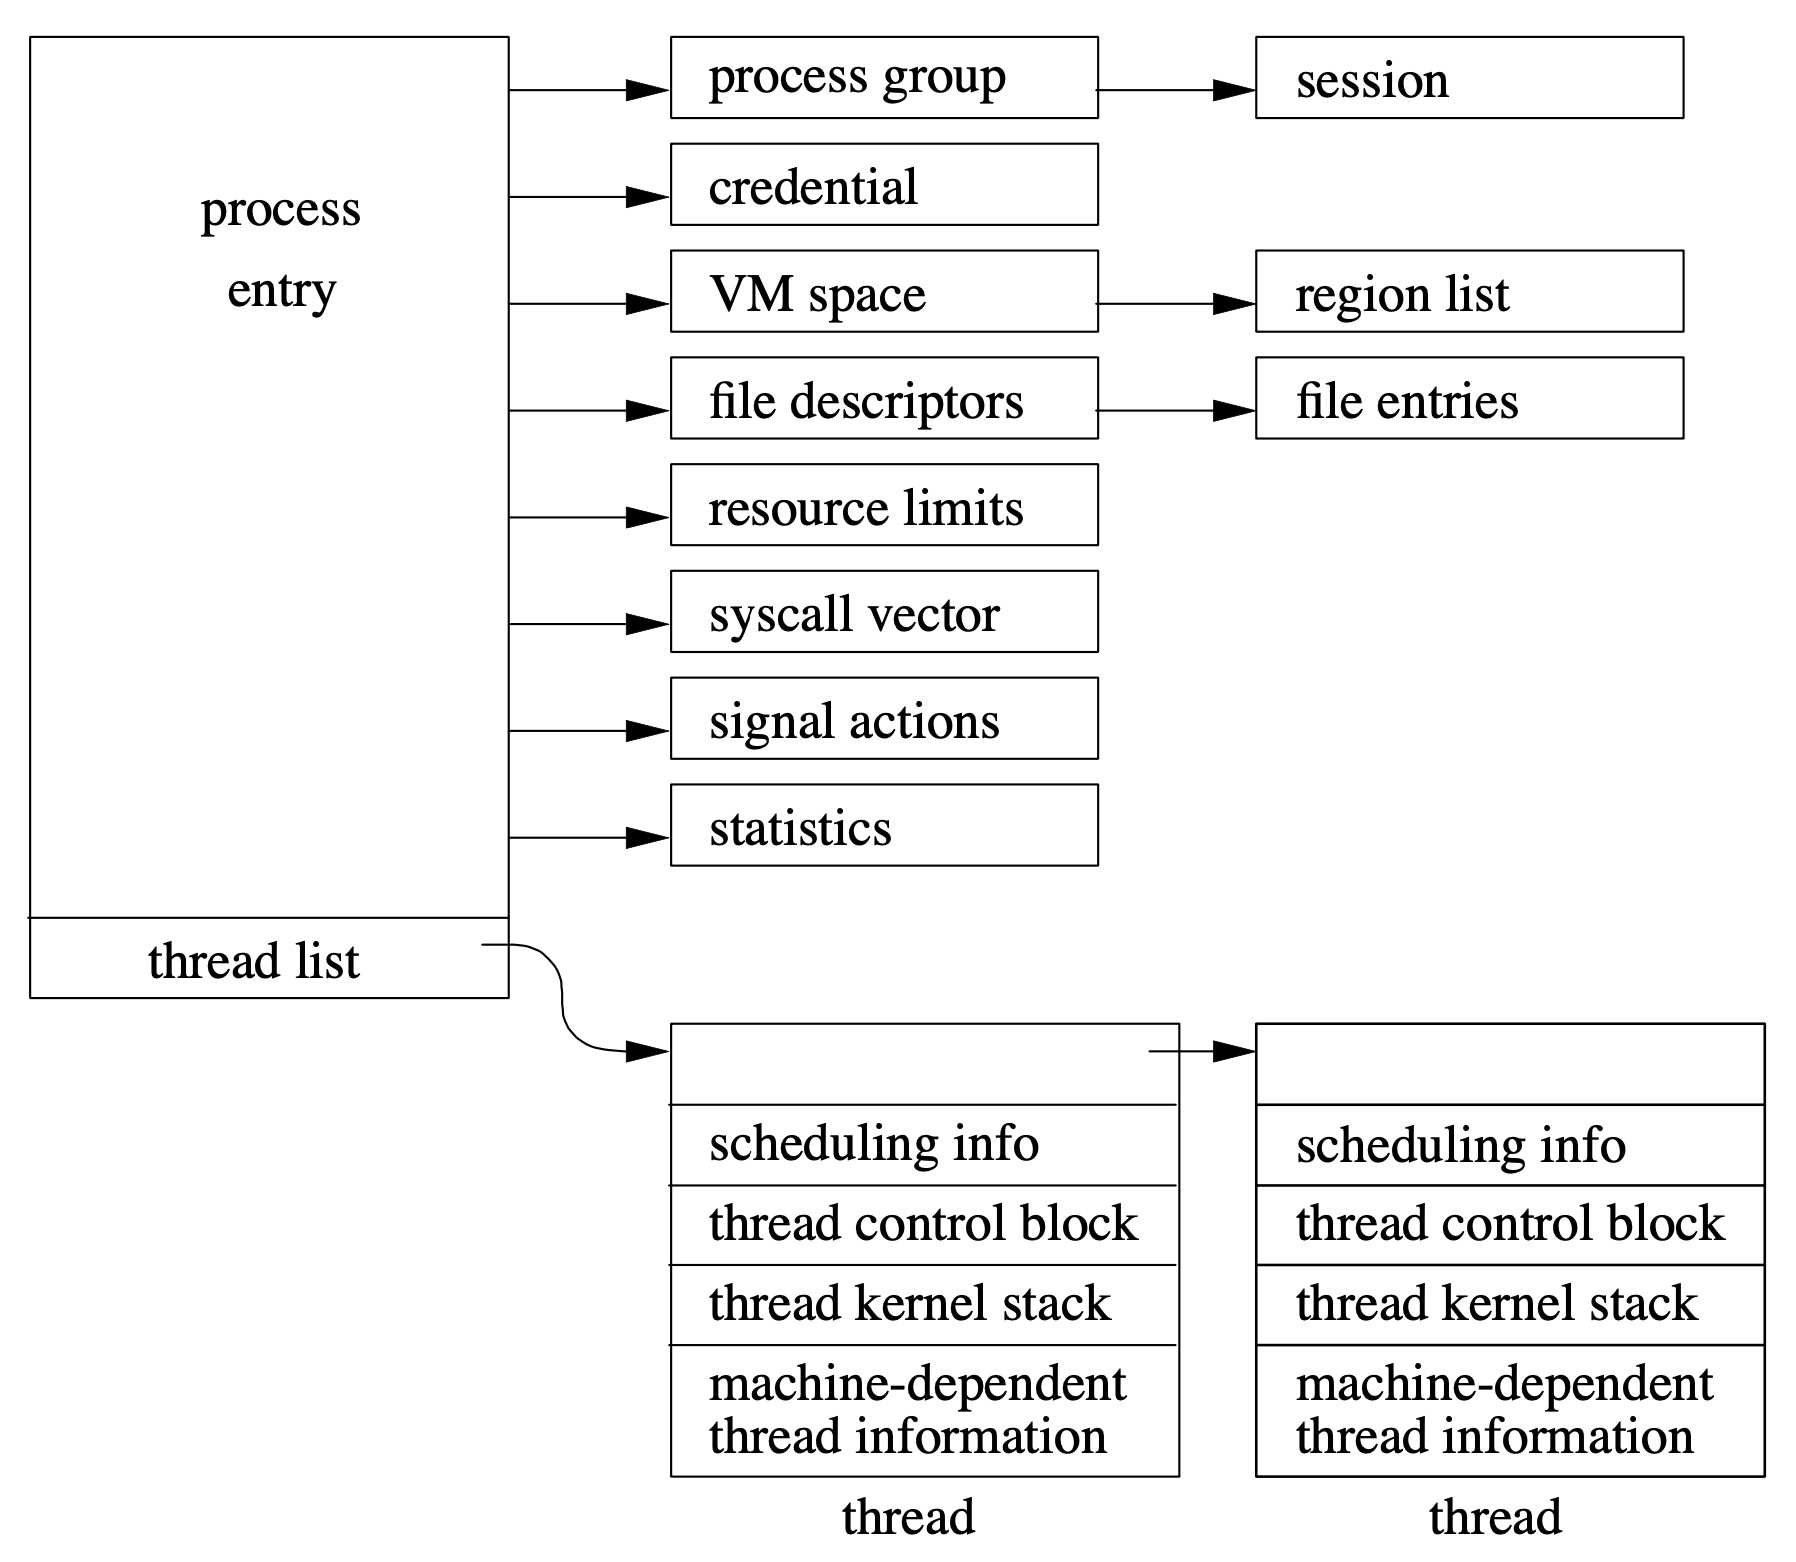
\includegraphics[width=0.6\textwidth]{images/processStructure.png}
    \caption{Estado del proceso.}
    \label{fig:process_state}
\end{figure}

\subsubsection{Estructura de hilos}
Un hilo es la unidad de ejecución de un proceso; necesita un espacio de direcciones y otros recursos, pero puede compartir muchos de ellos con otros hilos. Cuando varios hilos comparten un espacio de direcciones y otros recursos, son planificados de manera independiente y en FreeBSD, todos pueden ejecutar llamadas al sistema simultáneamente.\par

FreeBSD adopta el modelo 1:1, en el que cada hilo de usuario se corresponde con un hilo a nivel de kernel para mejorar la eficiencia de las aplicaciones.\par

La estructura de un hilo, que se muestra en la Figura~\ref{fig:process_state}, solo contiene la información necesaria para ejecutarse en el kernel del sistema operativo:

\begin{itemize}
    \item Información para la planificación: se refiere a la prioridad del hilo, la prioridad de planificación en modo usuario, la cantidad de tiempo que ha pasado durmiendo y el uso reciente de la CPU. Además, se indica el estado de ejecución del hilo, banderas de estado adicionales, y si el hilo está durmiendo, información sobre el canal y evento por el cual espera.
    \item TSB (thread state block): conjunto de registros definidos por la arquitectura de la máquina que se utiliza para gestionar la memoria y otros aspectos del procesamiento de datos. Incluye registros de propósito general, punteros de pila, contador de programa, palabra de estado del procesador y registros de gestión de memoria.
    \item Pila del kernel: pila para usar al ejecutar en el kernel. Las pilas del kernel deben mantenerse pequeñas para evitar desperdiciar memoria física.
    \item Estado de la máquina: se refiere a la información del hilo dependiente de la máquina.
\end{itemize}